\documentclass{article}
% Fernando Crema
% Master in Data Science - Sapienza Università di Roma
\usepackage{tikz}
\usetikzlibrary{automata,positioning}
\begin{document}

% Picture for HTT 

\vfill

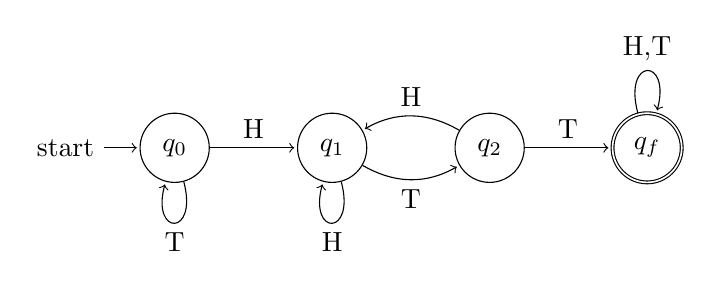
\begin{tikzpicture}[shorten >=1pt,node distance=2cm,on grid,auto] 
   \node[state,initial] (q_0)   {$q_0$}; 
   \node[state] (q_1) [right=of q_0] {$q_1$}; 
   \node[state] (q_2) [right=of q_1] {$q_2$}; 
   \node[state,accepting](q_f) [right=of q_2] {$q_f$};
    \path[->] 
    (q_0) edge  node {H} (q_1)
          edge [loop below] node {T} ()
    (q_1) edge [bend right] node [swap] {T} (q_2)
          edge [loop below] node {H} ()
    (q_2) edge  node {T} (q_f) 
          edge [bend right] node [swap] {H} (q_1)
    (q_f) edge [loop above] node {H,T} ();
\end{tikzpicture}

% Picture for HTH

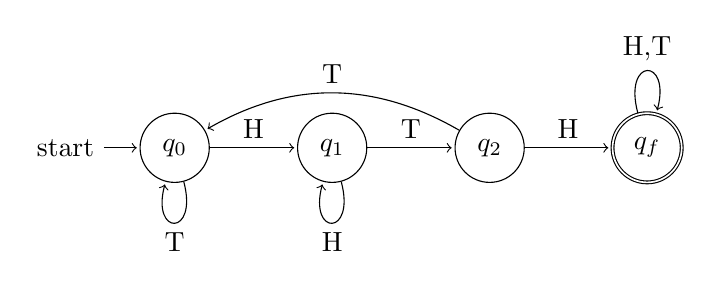
\begin{tikzpicture}[shorten >=1pt,node distance=2cm,on grid,auto] 
   \node[state,initial] (q_0)   {$q_0$}; 
   \node[state] (q_1) [right=of q_0] {$q_1$}; 
   \node[state] (q_2) [right=of q_1] {$q_2$}; 
   \node[state,accepting](q_f) [right=of q_2] {$q_f$};
    \path[->] 
    (q_0) edge  node {H} (q_1)
          edge [loop below] node {T} ()
    (q_1) edge  node  {T} (q_2)
          edge [loop below] node {H} ()
    (q_2) edge [bend right] node [swap] {T} (q_0) 
          edge node {H} (q_f)
    (q_f) edge [loop above] node {H,T} ();
\end{tikzpicture}
\end{document}  